\documentclass{standalone}

\usepackage{tikz}


\usepackage[utf8]{inputenc}
\usepackage{cmap}

\usepackage[english]{babel}

% \usepackage{amsthm}


\usepackage{amsmath}
\usepackage{amssymb}
\usepackage{dsfont}
\usepackage{mathrsfs}

\usepackage{hyperref}
%\usepackage[a4paper,hmargin=1.5in,vmargin=1.5in]{geometry}
\hypersetup{colorlinks = true, urlcolor = blue, linkcolor = blue, citecolor = red}
\usepackage{cleveref}

\usepackage{graphicx} % including pictures
\usepackage[export]{adjustbox} % use max width and max height for figures


\usepackage{caption}
\captionsetup[table]{format=hang,justification=raggedright,position=bottom,skip=15pt,textfont={sl},labelfont={bf}}
\captionsetup[figure]{format=hang,justification=raggedright,position=bottom,skip=15pt,textfont={sl},labelfont={bf}}

\usepackage{algorithm}
\usepackage{algpseudocode}
\algnewcommand{\LineComment}[1]{\State{\color{gray} \(\triangleright\) #1}}
\usepackage{listings}
\usepackage{pgfplots}
\usepackage{subcaption}
\usepackage{graphicx}
\usepackage{tikz}
\usetikzlibrary{decorations.pathreplacing}
\usetikzlibrary{arrows}
\usetikzlibrary{arrows.meta}
\usetikzlibrary{patterns}
\usetikzlibrary{shapes}
\usetikzlibrary{shadows}
\usetikzlibrary{calc}
\usetikzlibrary{math}
\tikzstyle{fun}=[draw,very thick,fill=white]
\tikzstyle{fork}=[shape=circle,inner sep=0pt,minimum size=3pt,fill=black]
\tikzstyle{op}=[inner sep=2pt]

\usepackage{ifthen}
\usepackage{comment}

\usepackage{booktabs}
\usepackage{multirow}
\usepackage{colortbl}
\usepackage{multicol} % To have lists over multiple columns

\usepackage{color,soul} % \st strikeout, \hl hilight

% To use monospace font in arrays easily
\usepackage{array}
\newcolumntype{t}{>{\tt}c}

\newcommand\todo[1]{{\color{red}\textbf{TODO:} #1}}

% \theoremstyle{theorem}
% \newtheorem{theorem}{Theorem}
% \newtheorem{maintheorem}{Main Theorem}
% \newtheorem{proposition}{Proposition}
% \newtheorem{conjecture}{Conjecture}
% \newtheorem{observation}{Observation}
% \newtheorem{goal}{Goal}
% \newtheorem{lemma}{Lemma}
% \newtheorem{corollary}{Corollary}
% \newtheorem{openproblem}{Open Problem}

% \theoremstyle{definition}
% \newtheorem{definition}{Definition}
% \newtheorem{caution}{Caution}

% \theoremstyle{remark}
% \newtheorem{remark}{Remark}

\definecolor{colorE}{RGB}{180,100,250}
\definecolor{colorE-1}{RGB}{100,100,250}
\definecolor{colorQi}{RGB}{250,100,100}
\definecolor{colorQf}{RGB}{250,100,180}
\definecolor{colorP}{RGB}{250,200,150}

\definecolor{colorM}{RGB}{200,120,255}
\definecolor{colorH}{RGB}{90,150,255}


\newcommand\diffusion{\mathcal{M}}
\newcommand\diffusionX{\mathcal{M}_x}
\newcommand\diffusionY{\mathcal{M}_y}
\newcommand\addition{\mathcal{A}}
\newcommand\sboxes{\mathcal{S}}
\newcommand\butterflyOpen{\mathcal{H}}
\newcommand\butterflyClosed{\mathcal{V}}
\newcommand\feedforward{\mathcal{F}}
\newcommand\feedforwardX{\mathcal{F}_x}
\newcommand\feedforwardY{\mathcal{F}_y}

\newcommand\pht{\mathcal{P}}


\newcommand\constraints{\emph{\color{red}+1}}

\newcommand\LL{\mathcal{L}}
\newcommand\Z{\mathcal{Z}}
\newcommand\complex{\mathbb{C}}
\newcommand\F{\mathbb{F}}
\newcommand\ftwo{\mathbb{F}_2}
\newcommand\field[1]{\mathbb{F}_{#1}}
\newcommand\Zmod[1]{\mathbb{Z}/ {#1} \mathbb{Z}}
\newcommand\proba[1]{\mathrm{Pr}\left[ #1  \right]}
\newcommand\bigoh{\mathrm{O}}
\newcommand\trace{\mathrm{Tr}}
\newcommand\traceSub[1]{\mathrm{Tr}_{#1}}
\newcommand\charac[1]{\mathds{1}_{#1}}
\newcommand\nwidth{t}


\newcommand\xor{\textsc{xor}}
\newcommand\xored{\textsc{xor}ed}
\newcommand\xors{\textsc{xor}s}
\newcommand\Tand{\textsc{And}}
\newcommand\Tands{\textsc{And}s}

\newcommand\kronecker[2]{\hat{\delta}\left( #1, #2 \right)}
\newcommand\scalarprod[2]{\left\langle #1, #2 \right\rangle}
\newcommand\walsh[1]{\mathcal{W}_{#1}}
\newcommand\fourier[1]{\mathcal{W}_{#1}}
\newcommand\ddt[1]{\delta_{#1}}
\newcommand\identity{\mathcal{I}}
\newcommand\hw{\mathrm{hw}}
\newcommand\hweight[1]{\mathrm{hw}\left( #1 \right)}
\newcommand\coveredby{\preccurlyeq}
\newcommand\lat[1]{\mathcal{W}_{#1}}

\newcommand\ind[2]{\mathbf{1}_{#1}\left( #2 \right)}

\newcommand\closedbutterfly[3]{\mathsf{V}^{#1}_{#2, #3}}
\newcommand\openbutterfly[3]{\mathsf{H}^{#1}_{#2, #3}}
\newcommand\newbutterfly[1]{\mathsf{N}_{#1}}
\newcommand\linearspan[1]{\langle #1 \rangle}
\newcommand\rank{\mathrm{rank}}
\newcommand\extract[1]{\mathcal{X}_{#1}}
\newcommand\walshZeroes[1]{\mathcal{Z}_{#1}}
\newcommand\ddtZeroes[1]{\mathcal{Z}^D_{#1}}



% \newcommand\jacobian[2]{\mathrm{Jac}_{#2}#1}
\newcommand\jacobian[2]{\mathrm{Jac}\ \! #1 (#2)}
\newcommand\Jlin[2]{\mathrm{Jac}_{\rm lin}\ \! #1 (#2)}
\newcommand\partialDiff[2]{\frac{\partial #1}{\partial #2}}

\newcommand\permSet[1]{\mathfrak{S}_{#1}}

\newcommand{\GL}[2]{\mathbf{GL}_{#1}(#2)}

\newcommand{\ff}[1]{\mathbb{F}_{#1}} % finite field
\newcommand\comatrice{\mathsf{Cof}}
\newtheorem{modeling}{Modeling}
\newtheorem{conj}{Conjecture}
\newtheorem{conv}{Convention}
\newtheorem{cor}{Corollary}
\newtheorem{ass}{Assumption}
\newtheorem{esti}{Estimate}

\begin{document}

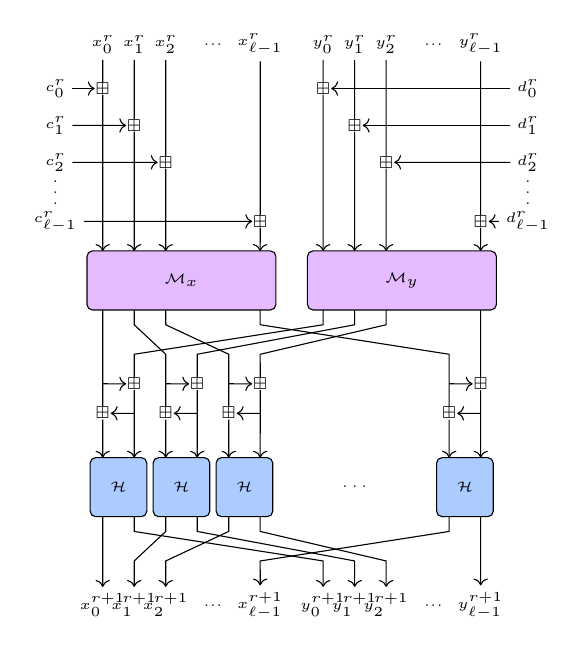
\begin{tikzpicture}[xscale=0.4,yscale=0.75]
  \tiny
  \begin{scope}[xshift=0cm]
	  \node (x0) at (0.5, 0.5) {$x_{0}^r$} ;
	  \node (x1) at (1.5, 0.5) {$x_{1}^r$} ;
	  \node (x2) at (2.5, 0.5) {$x_{2}^r$} ;
	  \node at (4, 0.5) {$...$} ;
	  \node (xl) at (5.5, 0.5) {$x_{\ell-1}^r$} ;
	  
	  \node (c0) at (-1, -0.25) {$c_0^r$} ;
	  \node (c1) at (-1, -0.875) {$c_1^r$} ;
	  \node (c2) at (-1, -1.5) {$c_2^r$} ;
	  \node at (-1, -1.875) {$\vdots$} ;
	  \node (cl) at (-1, -2.5) {$c_{\ell-1}^r$} ;
	  
	  \node[inner sep=0] (addx0) at (0.5, -0.25) {$\boxplus$} ;
	  \node[inner sep=0] (addx1) at (1.5, -0.875) {$\boxplus$} ;
	  \node[inner sep=0] (addx2) at (2.5, -1.5) {$\boxplus$} ;
	  \node[inner sep=0] (addxl) at (5.5, -2.5) {$\boxplus$} ;
	  
	  \draw[->] (x0) -- (addx0) -- (0.5, -3);
	  \draw[->] (c0) -- (addx0);

	  \draw[->] (x1) -- (addx1) -- (1.5, -3);
	  \draw[->] (c1) -- (addx1);

	  \draw[->] (x2) -- (addx2) -- (2.5, -3);
	  \draw[->] (c2) -- (addx2);

	  \draw[->] (xl) -- (addxl) -- (5.5, -3);
	  \draw[->] (cl) -- (addxl);

	  \node (u0) at (0.5, -9) {$x_{0}^{r+1}$} ;
	  \node (u1) at (1.5, -9) {$x_{1}^{r+1}$} ;
	  \node (u2) at (2.5, -9) {$x_{2}^{r+1}$} ;
	  \node at (4, -9) {$...$} ;
	  \node (ul) at (5.5, -9) {$x_{\ell-1}^{r+1}$} ;

	  \draw[rounded corners=2pt,fill=colorM!50] (0, -4) rectangle (6, -3) node[pos=0.5]{$\diffusionX$} ;
  \end{scope}

  \begin{scope}[xshift=7cm]
	  \node (y0) at (0.5, 0.5) {$y_{0}^r$} ;
	  \node (y1) at (1.5, 0.5) {$y_{1}^r$} ;
	  \node (y2) at (2.5, 0.5) {$y_{2}^r$} ;
	  \node at (4, 0.5) {$...$} ;
	  \node (yl) at (5.5, 0.5) {$y_{\ell-1}^r$} ;
	  
	  \node (d0) at (7, -0.25) {$d_0^r$} ;
	  \node (d1) at (7, -0.875) {$d_1^r$} ;
	  \node (d2) at (7, -1.5) {$d_2^r$} ;
	  \node at (7, -1.875) {$\vdots$} ;
	  \node (dl) at (7, -2.5) {$d_{\ell-1}^r$} ;

	  \node[inner sep=0] (addy0) at (0.5, -0.25) {$\boxplus$} ;
	  \node[inner sep=0] (addy1) at (1.5, -0.875) {$\boxplus$} ;
	  \node[inner sep=0] (addy2) at (2.5, -1.5) {$\boxplus$} ;
	  \node[inner sep=0] (addyl) at (5.5, -2.5) {$\boxplus$} ; 
	  
	  \draw[->] (y0) -- (addy0) -- (0.5, -3);
	  \draw[->] (d0) -- (addy0);

	  \draw[->] (y1) -- (addy1) -- (1.5, -3);
	  \draw[->] (d1) -- (addy1);

	  \draw[->] (y2) -- (addy2) -- (2.5, -3);
	  \draw[->] (d2) -- (addy2);
 
	  \draw[->] (yl) -- (addyl) -- (5.5, -3);
	  \draw[->] (dl) -- (addyl);

	  \node (v0) at (0.5, -9) {$y_{0}^{r+1}$} ;
	  \node (v1) at (1.5, -9) {$y_{1}^{r+1}$} ;
	  \node (v2) at (2.5, -9) {$y_{2}^{r+1}$} ;
	  \node at (4, -9) {$...$} ;
	  \node (vl) at (5.5, -9) {$y_{\ell-1}^{r+1}$} ;

	  \draw[rounded corners=2pt,fill=colorM!50] (0, -4) rectangle (6, -3) node[pos=0.5]{$\diffusionY$} ;
  \end{scope}


	% Before S-box %

  	\node[inner sep=0] (add1x) at (0.5, -5.75) {$\boxplus$} ;
  	\node[inner sep=0] (add1y) at (1.5, -5.25) {$\boxplus$} ;

  	\node[inner sep=0] (add2x) at (2.5, -5.75) {$\boxplus$} ;
  	\node[inner sep=0] (add2y) at (3.5, -5.25) {$\boxplus$} ;

  	\node[inner sep=0] (add3x) at (4.5, -5.75) {$\boxplus$} ;
  	\node[inner sep=0] (add3y) at (5.5, -5.25) {$\boxplus$} ;

  	\node[inner sep=0] (addlx) at (11.5, -5.75) {$\boxplus$} ;
  	\node[inner sep=0] (addly) at (12.5, -5.25) {$\boxplus$} ;

  	%1st Flystel
	\draw[->] (0.5, -4) -- (add1x) -- (0.5, -6.5) ;
	\draw[->] (7.5, -4) -- (7.5, -4.25) -- (1.5, -4.75) -- (add1y) -- (1.5, -6.5);
	\draw[->] (0.5, -5.25) -- (add1y);
	\draw[->] (1.5, -5.75) -- (add1x);

	%2nd Flystel
	\draw[->] (1.5, -4) -- (1.5, -4.25) -- (2.5, -4.75) -- (add2x) -- (2.5, -6.5) ;
	\draw[->] (8.5, -4) -- (8.5, -4.25) -- (3.5, -4.75) -- (add2y) -- (3.5, -6.5);
	\draw[->] (2.5, -5.25) -- (add2y);
	\draw[->] (3.5, -5.75) -- (add2x);

	%3rd Flystel
	\draw[->] (2.5, -4) -- (2.5, -4.25) -- (4.5, -4.75) -- (add3x) -- (4.5, -6.5) ;
	\draw[->] (9.5, -4) -- (9.5, -4.25) -- (5.5, -4.75) -- (add3y) -- (5.5, -6.5);
	\draw[->] (4.5, -5.25) -- (add3y);
	\draw[->] (5.5, -5.75) -- (add3x);

	%last Flystel
	\draw[->] (5.5, -4) -- (5.5, -4.25) -- (11.5, -4.75) -- (addlx) -- (11.5, -6.5);
	\draw[->] (12.5, -4) -- (addly) -- (12.5, -6.5) ;
	\draw[->] (11.5, -5.25) -- (addly);
	\draw[->] (12.5, -5.75) -- (addlx);

	\draw[rounded corners=2pt,fill=colorH!50] (0.1, -7.5) rectangle node {$\butterflyOpen$} (1.9, -6.5) ;
	\draw[rounded corners=2pt,fill=colorH!50] (2.1, -7.5) rectangle node {$\butterflyOpen$} (3.9, -6.5) ;
	\draw[rounded corners=2pt,fill=colorH!50] (4.1, -7.5) rectangle node {$\butterflyOpen$} (5.9, -6.5) ;
	\draw[rounded corners=2pt,fill=colorH!50] (11.1, -7.5) rectangle node {$\butterflyOpen$} (12.9, -6.5) ;
	
	\node at (8.5,-7) {$\ldots$};
	
	% After S-box %

	%1st Flystel
	\draw[->] (0.5, -7.5) -- (u0) ;
	\draw[->] (1.5, -7.5) -- (1.5, -7.75) -- (7.5, -8.25) -- (v0);
	
	%2nd Flystel
	\draw[->] (2.5, -7.5) -- (2.5, -7.75) -- (1.5, -8.25) -- (u1);
	\draw[->] (3.5, -7.5) -- (3.5, -7.75) -- (8.5, -8.25) -- (v1);

	%3rd Flystel
	\draw[->] (4.5, -7.5) -- (4.5, -7.75) -- (2.5, -8.25) -- (u2);
	\draw[->] (5.5, -7.5) -- (5.5, -7.75) -- (9.5, -8.25) -- (v2);

	%last Flystel
	\draw[->] (11.5, -7.5) -- (11.5, -7.75) -- (5.5, -8.25) -- (ul) ;
	\draw[->] (12.5, -7.5) -- (vl) ;

\end{tikzpicture}


\end{document}
